\subsection{From physics to computation}
To be able to do a reservoir simulation, we start with a physicist who model fluid flow inside porous medium.
%
Most of models are based on three physical equations, the conservation of mass, ideal gas law and Darcy's law.
%
Then we discretize the reservoir into cells with a finite volume schema.
%
For each cell of the reservoir, we can compute a non-linear equation of each primary variables (e.g.: pressure, oil saturation).
%
To solve the non-linear systems of equation, we use the Newton–Raphson method.
%
This method is iterative, we begins with an initial guess $X_0$ reasonably close to the solution $X_n$ which satisfied $F(X_n) = 0$.

%   (-_-)   %
\begin{figure}[!ht]
  \centering
  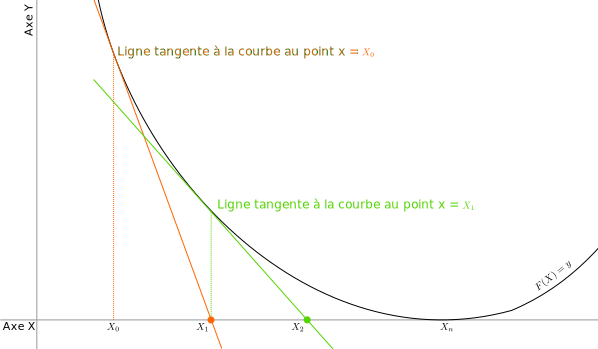
\includegraphics[width=0.8\textwidth]{newton}
  \caption{Example of two Newton steps in one dimension space.
    Each tangent lines correspond to a linear equation to solve.
    We want to find $X_n$ and we start with $X_0$.}
\label{fig:newton}
\end{figure}

The example in the figure~\ref{fig:newton} is only in one dimension but it's quite the same approach that can be done when we work with an arbitrary number of dimensions.
%
Linear equations of reservoir simulation can be represented as large sparse matrices, in which each row represents all interactions between an element and its direct neighbors.
%
So in a 3D regular mesh, there can have up to seven interactions per row.
%
Each interaction is represented by a small square matrix of the size of the number of primary variables.
%
Sparse linear algebra solvers, like GMRES, are then used to solve all linear problems use in the Newton method.
